
\begin{figure}[t]
\centering
\begin{tikzpicture}
    \begin{customlegend}[legend columns=3,
        legend entries={\sketragp, \sketragu, \hybridrag}
        ,
        legend style={at={(0.45,1.05)},anchor=north,draw=none,font=\footnotesize,column sep=0.1cm}]
    \addlegendimage{line width=0.3mm,mark size=2pt,mark=o,color=Red}
    \addlegendimage{line width=0.3mm,mark size=2pt,mark=x,color=Orange}
    \addlegendimage{line width=0.3mm,mark size=2pt,mark=pentagon,color=Green}
    \end{customlegend}
\end{tikzpicture}
\\
\subfloat[MuSiQue]{
\hspace{-1.2mm}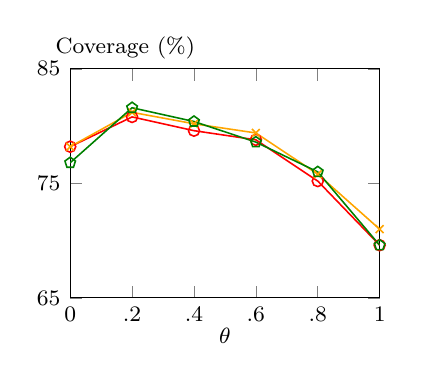
\begin{tikzpicture}[scale=1]
    \begin{axis}[
        height=\columnwidth/2.7,
        width=\columnwidth/2.2,
        ylabel={Coverage (\%)},
        xlabel={$\theta$},
        xmin=0.0, xmax=1.0,
        ymin=0.65, ymax=0.85,
        xtick={0, 0.2, 0.4, 0.6, 0.8, 1.0},
        xticklabel style = {font=\footnotesize},
        xticklabels={0, .2, .4, .6, .8, 1},
        ytick={0.65,0.75,0.85},
        yticklabels={65,75,85},
        every axis y label/.style={at={(current axis.north west)},right=7mm,above=0mm},
        label style={font=\footnotesize},
        tick label style={font=\footnotesize},
        every axis x label/.style={at={(current axis.south)},right=0mm,above=-7mm},
        label style={font=\footnotesize},
        tick label style={font=\footnotesize},
    ]

%     \addplot[line width=0.2mm,mark size=2pt,mark=o,color=Red]
%         plot coordinates { % SkeTRAG - 1200
% (0, 0.176300934)
% (0.2, 0.188094157)
% (0.4, 0.196128801)
% (0.6, 0.1876783)
% (0.8, 0.19700453)
% (1.0, 0.157561628)
%     };

%     \addplot[line width=0.2mm,mark size=2pt,mark=o,color=Red!75]
%         plot coordinates { % SkeTRAG - 600
% (0, 0.170179462)
% (0.2, 0.240968426)
% (0.4, 0.226319961)
% (0.6, 0.232188549)
% (0.8, 0.229216351)
% (1.0, 0.208775333)
%     };

%     \addplot[line width=0.2mm,mark size=2pt,mark=o,color=Red!50]
%         plot coordinates { % SkeTRAG - 300
% (0, 0.169292118)
% (0.2, 0.24154141)
% (0.4, 0.256892671)
% (0.6, 0.255549124)
% (0.8, 0.266975679)
% (1.0, 0.256770818)
%     };

    \addplot[line width=0.2mm,mark size=2pt,mark=o,color=Red]
        plot coordinates { % SkeTRAG - 150
(0.0, 0.782)
(0.2, 0.808)
(0.4, 0.796)
(0.6, 0.788)
(0.8, 0.752)
(1.0, 0.696)
    };

    \addplot[line width=0.2mm,mark size=2pt,mark=x,color=Orange]
        plot coordinates { % SkeTRAG - uniform
(0.0, 0.782)
(0.2, 0.812)
(0.4, 0.802)
(0.6, 0.794)
(0.8, 0.758)
(1.0, 0.71)
    };

    \addplot[line width=0.2mm,mark size=2pt,mark=pentagon,color=Green]
        plot coordinates { % Hybrid
(0.0, 0.768)
(0.2, 0.816)
(0.4, 0.804)
(0.6, 0.786)
(0.8, 0.76)
(1.0, 0.696)
    };



\end{axis}

\end{tikzpicture}
\hspace{-1.2mm}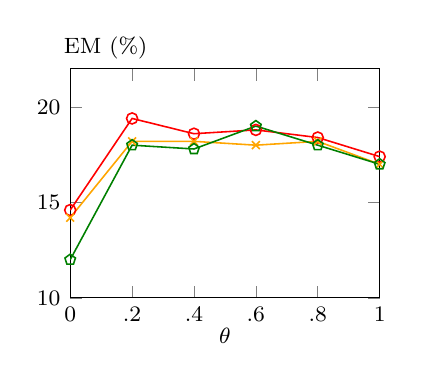
\begin{tikzpicture}[scale=1]
    \begin{axis}[
        height=\columnwidth/2.7,
        width=\columnwidth/2.2,
        ylabel={EM (\%)},
        xlabel={$\theta$},
        xmin=0.0, xmax=1.0,
        ymin=0.1, ymax=0.22,
        xtick={0, 0.2, 0.4, 0.6, 0.8, 1.0},
        xticklabel style = {font=\footnotesize},
        xticklabels={0, .2, .4, .6, .8, 1},
        ytick={0.10, 0.15,0.2},
        yticklabels={10, 15, 20},
        every axis y label/.style={at={(current axis.north west)},right=4.5mm,above=0mm},
        label style={font=\footnotesize},
        tick label style={font=\footnotesize},
        every axis x label/.style={at={(current axis.south)},right=0mm,above=-7mm},
        label style={font=\footnotesize},
        tick label style={font=\footnotesize},
    ]

%     \addplot[line width=0.2mm,mark size=2pt,mark=o,color=Red]
%         plot coordinates { % SkeTRAG
% (0, 0.122)
% (0.2, 0.132)
% (0.4, 0.144)
% (0.6, 0.134)
% (0.8, 0.14)
% (1.0, 0.114)
%     };

%     \addplot[line width=0.2mm,mark size=2pt,mark=o,color=Red!75]
%         plot coordinates { % SkeTRAG - 600
% (0, 0.108)
% (0.2, 0.174)
% (0.4, 0.17)
% (0.6, 0.172)
% (0.8, 0.166)
% (1.0, 0.152)
%     };

%     \addplot[line width=0.2mm,mark size=2pt,mark=o,color=Red!50]
%         plot coordinates { % SkeTRAG - 300
% (0, 0.104)
% (0.2, 0.176)
% (0.4, 0.192)
% (0.6, 0.186)
% (0.8, 0.198)
% (1.0, 0.192)
%     };

    \addplot[line width=0.2mm,mark size=2pt,mark=o,color=Red]
        plot coordinates { % SkeTRAG - 150
(0, 0.146)
(0.2, 0.194)
(0.4, 0.186)
(0.6, 0.188)
(0.8, 0.184)
(1.0, 0.174)
    };

    \addplot[line width=0.2mm,mark size=2pt,mark=x,color=Orange]
        plot coordinates { % SkeTRAG - uniform
(0.0, 0.142)
(0.2, 0.182)
(0.4, 0.182)
(0.6, 0.18)
(0.8, 0.182)
(1.0, 0.17)
    };


    \addplot[line width=0.2mm,mark size=2pt,mark=pentagon,color=Green]
        plot coordinates { % Hybrid
(0.0, 0.12)
(0.2, 0.18)
(0.4, 0.178)
(0.6, 0.19)
(0.8, 0.18)
(1.0, 0.17)
    };
    
    \end{axis}

\end{tikzpicture}
\hspace{-1.2mm}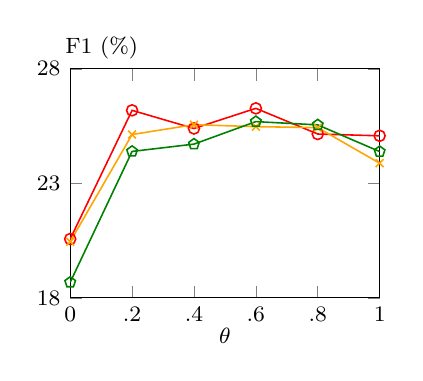
\begin{tikzpicture}[scale=1]
    \begin{axis}[
        height=\columnwidth/2.7,
        width=\columnwidth/2.2,
        ylabel={F1 (\%)},
        xlabel={$\theta$},
        xmin=0.0, xmax=1.0,
        ymin=0.18, ymax=0.28,
        xtick={0, 0.2, 0.4, 0.6, 0.8, 1.0},
        xticklabel style = {font=\footnotesize},
        xticklabels={0, .2, .4, .6, .8, 1},
        ytick={0.18,0.23,0.28},
        yticklabels={18,23,28},
        every axis y label/.style={at={(current axis.north west)},right=4mm,above=0mm},
        label style={font=\footnotesize},
        tick label style={font=\footnotesize},
        every axis x label/.style={at={(current axis.south)},right=0mm,above=-7mm},
        label style={font=\footnotesize},
        tick label style={font=\footnotesize},
    ]

%     \addplot[line width=0.2mm,mark size=2pt,mark=o,color=Red]
%         plot coordinates { % SkeTRAG - 1200
% (0, 0.176300934)
% (0.2, 0.188094157)
% (0.4, 0.196128801)
% (0.6, 0.1876783)
% (0.8, 0.19700453)
% (1.0, 0.157561628)
%     };

%     \addplot[line width=0.2mm,mark size=2pt,mark=o,color=Red!75]
%         plot coordinates { % SkeTRAG - 600
% (0, 0.170179462)
% (0.2, 0.240968426)
% (0.4, 0.226319961)
% (0.6, 0.232188549)
% (0.8, 0.229216351)
% (1.0, 0.208775333)
%     };

%     \addplot[line width=0.2mm,mark size=2pt,mark=o,color=Red!50]
%         plot coordinates { % SkeTRAG - 300
% (0, 0.169292118)
% (0.2, 0.24154141)
% (0.4, 0.256892671)
% (0.6, 0.255549124)
% (0.8, 0.266975679)
% (1.0, 0.256770818)
%     };

    \addplot[line width=0.2mm,mark size=2pt,mark=o,color=Red]
        plot coordinates { % SkeTRAG - 150
(0, 0.205702525)
(0.2, 0.261869012)
(0.4, 0.253952005)
(0.6, 0.262738242)
(0.8, 0.251539304)
(1.0, 0.25075364)
    };

    \addplot[line width=0.2mm,mark size=2pt,mark=x,color=Orange]
        plot coordinates { % SkeTRAG - uniform
(0.0, 0.204517181)
(0.2, 0.251324036)
(0.4, 0.255602241)
(0.6, 0.254754718)
(0.8, 0.254316549)
(1.0, 0.238788916)
    };

    \addplot[line width=0.2mm,mark size=2pt,mark=pentagon,color=Green]
        plot coordinates { % Hybrid
(0.0, 0.186808122)
(0.2, 0.243938036)
(0.4, 0.247127927)
(0.6, 0.256951852)
(0.8, 0.255521173)
(1.0, 0.243875902)
    };

\end{axis}

\end{tikzpicture}
}%
\\
\subfloat[Hotpot]{
\hspace{-1.2mm}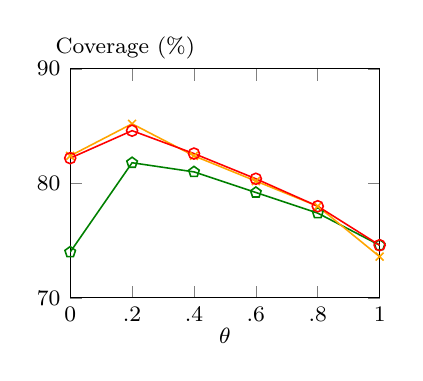
\begin{tikzpicture}[scale=1]
    \begin{axis}[
        height=\columnwidth/2.7,
        width=\columnwidth/2.2,
        ylabel={Coverage (\%)},
        xlabel={$\theta$},
        xmin=0.0, xmax=1.0,
        ymin=0.7, ymax=0.9,
        xtick={0, 0.2, 0.4, 0.6, 0.8, 1.0},
        xticklabel style = {font=\footnotesize},
        xticklabels={0, .2, .4, .6, .8, 1},
        ytick={0.7,0.8,0.9},
        yticklabels={70,80,90},
        every axis y label/.style={at={(current axis.north west)},right=7mm,above=0mm},
        label style={font=\footnotesize},
        tick label style={font=\footnotesize},
        every axis x label/.style={at={(current axis.south)},right=0mm,above=-7mm},
        label style={font=\footnotesize},
        tick label style={font=\footnotesize},
    ]

%     \addplot[line width=0.2mm,mark size=2pt,mark=o,color=Red]
%         plot coordinates { % SkeTRAG - 1200
% (0, 0.413087256)
% (0.2, 0.404018972)
% (0.4, 0.389217444)
% (0.6, 0.389989153)
% (0.8, 0.381677978)
% (1.0, 0.301755047)
%     };

    \addplot[line width=0.2mm,mark size=2pt,mark=pentagon,color=Green]
        plot coordinates { % Hybrid
(0.0, 0.74)
(0.2, 0.818)
(0.4, 0.81)
(0.6, 0.792)
(0.8, 0.774)
(1.0, 0.746)
    };

    \addplot[line width=0.2mm,mark size=2pt,mark=x,color=DeepBlue]
        plot coordinates { % Skeleton

    };

%     \addplot[line width=0.2mm,mark size=2pt,mark=o,color=Red!75]
%         plot coordinates { % SkeTRAG - 600
% (0, 0.412137776)
% (0.2, 0.419856672)
% (0.4, 0.422807675)
% (0.6, 0.437430286)
% (0.8, 0.419080537)
% (1.0, 0.382516896)
%     };

%     \addplot[line width=0.2mm,mark size=2pt,mark=o,color=Red!50]
%         plot coordinates { % SkeTRAG - 300
% (0, 0.437839957)
% (0.2, 0.468297635)
% (0.4, 0.448441971)
% (0.6, 0.443180885)
% (0.8, 0.44557756)
% (1.0, 0.411810544)
%     };

    \addplot[line width=0.2mm,mark size=2pt,mark=x,color=Orange]
        plot coordinates { % SkeTRAG - uniform
(0.0, 0.824)
(0.2, 0.852)
(0.4, 0.824)
(0.6, 0.802)
(0.8, 0.78)
(1.0, 0.736)
    };

    \addplot[line width=0.2mm,mark size=2pt,mark=o,color=Red]
        plot coordinates { % SkeTRAG - 150
(0.0, 0.822)
(0.2, 0.846)
(0.4, 0.826)
(0.6, 0.804)
(0.8, 0.78)
(1.0, 0.746)
    };



    
    \end{axis}

\end{tikzpicture}
\hspace{-1.2mm}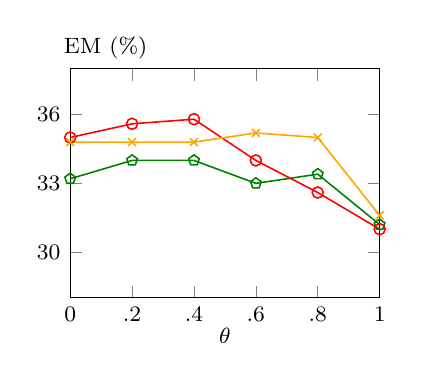
\begin{tikzpicture}[scale=1]
    \begin{axis}[
        height=\columnwidth/2.7,
        width=\columnwidth/2.2,
        ylabel={EM (\%)},
        xlabel={$\theta$},
        xmin=0.0, xmax=1.0,
        ymin=0.28, ymax=0.38,
        xtick={0, 0.2, 0.4, 0.6, 0.8, 1.0},
        xticklabel style = {font=\footnotesize},
        xticklabels={0, .2, .4, .6, .8, 1},
        ytick={0.30, 0.33, 0.36},
        yticklabels={30, 33, 36},
        every axis y label/.style={at={(current axis.north west)},right=4.5mm,above=0mm},
        label style={font=\footnotesize},
        tick label style={font=\footnotesize},
        every axis x label/.style={at={(current axis.south)},right=0mm,above=-7mm},
        label style={font=\footnotesize},
        tick label style={font=\footnotesize},
    ]

%     \addplot[line width=0.2mm,mark size=2pt,mark=o,color=Red]
%         plot coordinates { % SkeTRAG
% (0, 0.298)
% (0.2, 0.296)
% (0.4, 0.288)
% (0.6, 0.288)
% (0.8, 0.282)
% (1.0, 0.216)
%     };

    \addplot[line width=0.2mm,mark size=2pt,mark=pentagon,color=Green]
        plot coordinates { % Hybrid
(0.0, 0.332)
(0.2, 0.34)
(0.4, 0.34)
(0.6, 0.33)
(0.8, 0.334)
(1.0, 0.312)
    };

%     \addplot[line width=0.2mm,mark size=2pt,mark=o,color=Red!75]
%         plot coordinates { % SkeTRAG - 600
% (0, 0.3)
% (0.2, 0.312)
% (0.4, 0.322)
% (0.6, 0.33)
% (0.8, 0.318)
% (1.0, 0.284)
%     };

%     \addplot[line width=0.2mm,mark size=2pt,mark=o,color=Red!50]
%         plot coordinates { % SkeTRAG - 300
% (0, 0.322)
% (0.2, 0.346)
% (0.4, 0.338)
% (0.6, 0.336)
% (0.8, 0.336)
% (1.0, 0.312)
%     };

    \addplot[line width=0.2mm,mark size=2pt,mark=o,color=Red]
        plot coordinates { % SkeTRAG - 150
(0, 0.35)
(0.2, 0.356)
(0.4, 0.358)
(0.6, 0.34)
(0.8, 0.326)
(1.0, 0.31)
    };

    \addplot[line width=0.2mm,mark size=2pt,mark=x,color=Orange]
        plot coordinates { % SkeTRAG - uniform
(0.0, 0.348)
(0.2, 0.348)
(0.4, 0.348)
(0.6, 0.352)
(0.8, 0.350)
(1.0, 0.316)
    };
    
    \end{axis}

\end{tikzpicture}
\hspace{-1.2mm}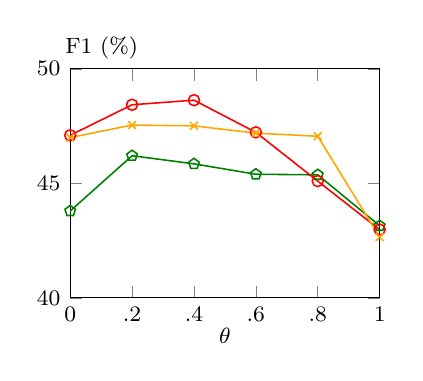
\begin{tikzpicture}[scale=1]
    \begin{axis}[
        height=\columnwidth/2.7,
        width=\columnwidth/2.2,
        ylabel={F1 (\%)},
        xlabel={$\theta$},
        xmin=0.0, xmax=1.0,
        ymin=0.4, ymax=0.5,
        xtick={0, 0.2, 0.4, 0.6, 0.8, 1.0},
        xticklabel style = {font=\footnotesize},
        xticklabels={0, .2, .4, .6, .8, 1},
        ytick={0.4, 0.45, 0.5},
        yticklabels={40, 45, 50},
        every axis y label/.style={at={(current axis.north west)},right=4mm,above=0mm},
        label style={font=\footnotesize},
        tick label style={font=\footnotesize},
        every axis x label/.style={at={(current axis.south)},right=0mm,above=-7mm},
        label style={font=\footnotesize},
        tick label style={font=\footnotesize},
    ]

%     \addplot[line width=0.2mm,mark size=2pt,mark=o,color=Red]
%         plot coordinates { % SkeTRAG - 1200
% (0, 0.413087256)
% (0.2, 0.404018972)
% (0.4, 0.389217444)
% (0.6, 0.389989153)
% (0.8, 0.381677978)
% (1.0, 0.301755047)
%     };

    \addplot[line width=0.2mm,mark size=2pt,mark=pentagon,color=Green]
        plot coordinates { % Hybrid
(0.0, 0.437930177)
(0.2, 0.462061217)
(0.4, 0.458510645)
(0.6, 0.453968044)
(0.8, 0.453729208)
(1.0, 0.431479231)
    };

%     \addplot[line width=0.2mm,mark size=2pt,mark=x,color=DeepBlue]
%         plot coordinates { % Skeleton

%     };

%     \addplot[line width=0.2mm,mark size=2pt,mark=o,color=Red!75]
%         plot coordinates { % SkeTRAG - 600
% (0, 0.412137776)
% (0.2, 0.419856672)
% (0.4, 0.422807675)
% (0.6, 0.437430286)
% (0.8, 0.419080537)
% (1.0, 0.382516896)
%     };

%     \addplot[line width=0.2mm,mark size=2pt,mark=o,color=Red!50]
%         plot coordinates { % SkeTRAG - 300
% (0, 0.437839957)
% (0.2, 0.468297635)
% (0.4, 0.448441971)
% (0.6, 0.443180885)
% (0.8, 0.44557756)
% (1.0, 0.411810544)
%     };

    \addplot[line width=0.2mm,mark size=2pt,mark=o,color=Red]
        plot coordinates { % SkeTRAG - 150
(0, 0.470963143)
(0.2, 0.484303943)
(0.4, 0.486306113)
(0.6, 0.472271351)
(0.8, 0.450982308)
(1.0, 0.429801034)
    };

    \addplot[line width=0.2mm,mark size=2pt,mark=x,color=Orange]
        plot coordinates { % SkeTRAG - uniform
(0.0, 0.469989276)
(0.2, 0.475449933)
(0.4, 0.4751002065)
(0.6, 0.4719215465)
(0.8, 0.4705509015)
(1.0, 0.426568579)
    };


    \end{axis}

\end{tikzpicture}
}%
\vspace{-2mm}
\caption{Answer quality by varying $\theta$.} \label{fig:quality-theta}
\vspace{-2mm}
\end{figure}